
\documentclass[8pt]{article}
\usepackage{amsmath, amsfonts, amsthm, amssymb}  % Some math symbols
% \usepackage{fullpage}
\usepackage[a4paper, left=0.5in, right=0.5in, top=0.5in, bottom=0.5in]{geometry}
\usepackage{graphicx}
\usepackage[x11names, rgb]{xcolor}
\usepackage{graphicx}
\usepackage{tikz}
\usepackage{tcolorbox}
\usetikzlibrary{decorations,arrows,shapes}
\usepackage{float} % Add this package to control float placement
\usepackage{etoolbox}
\usepackage{enumerate}
\usepackage{listings}
\usepackage{algorithm}
\usepackage{algpseudocode}
\usepackage{caption}
\lstset{
    language=Python,           % Set the language of the code
    basicstyle=\footnotesize\ttfamily,
    keywordstyle=\color{blue}, % Set color for keywords
    commentstyle=\color{gray}, % Set color for comments
    stringstyle=\color{red},   % Set color for strings
    numbers=left,              % Display line numbers on the left
    numberstyle=\tiny\color{gray}, % Style for line numbers
    frame=single,              % Add a frame around the code
    breaklines=true            % Allow line breaking
}


\setlength{\parindent}{0pt}
\setlength{\parskip}{5pt plus 1pt}

\newcommand{\N}{\mathbb N}
\newcommand{\E}{\mathbb E}
\newcommand{\V}{Var}
\renewcommand{\P}{\mathbb P}
\newcommand{\f}{\frac}


\newcommand{\nopagenumbers}{
    \pagestyle{empty}
}

\def\indented#1{\list{}{}\item[]}
\let\indented=\endlist

\providetoggle{questionnumbers}
\settoggle{questionnumbers}{true}
\newcommand{\noquestionnumbers}{
    \settoggle{questionnumbers}{false}
}

\newcounter{questionCounter}
\newenvironment{question}[2][\arabic{questionCounter}]{%
    \addtocounter{questionCounter}{1}%
    \setcounter{partCounter}{0}%
    \vspace{.25in} \hrule \vspace{0.4em}%
        \noindent{\bf \iftoggle{questionnumbers}{#1: }{}#2}%
    \vspace{0.8em} \hrule \vspace{.10in}%
}{$ $\newpage}

\newcounter{partCounter}[questionCounter]
\renewenvironment{part}[1][\alph{partCounter}]{%
    \addtocounter{partCounter}{1}%
    \vspace{.10in}%
    \begin{indented}%
       {\bf (#1)} %
}{\end{indented}}

\def\show#1{\ifdefempty{#1}{}{#1\\}}

\newcommand{\header}{%
\begin{center}
    {\Large \show\myhwname}
    \show\myname
    \show\myemail
    \show\mysection
    \show\hwname
\end{center}}

\usepackage{hyperref} % for hyperlinks
\hypersetup{
    colorlinks=true,
    linkcolor=blue,
    filecolor=magenta,      
    urlcolor=blue,
}

%%%%%%%%%%%%%%%%% Identifying Information %%%%%%%%%%%%%%%%%
%% For 312, we'd rather you DIDN'T tell us who you are   %%
%% in your homework so that we're not biased when        %%
%% So, even if you fill this information in, it will not %%
%% show up in the document unless you uncomment \header  %%
%% below                                                 %%
%%%%%%%%%%%%%%%%%%%%%%%%%%%%%%%%%%%%%%%%%%%%%%%%%%%%%%%%%%%
\newcommand{\myhwname}{DS 298: Random Variates in Computation }
\newcommand{\myname}{Naman Pesricha }
\newcommand{\myemail}{namanp@iisc.ac.in}
\newcommand{\hwname}{\textbf{Work Assignment - 2}}
\newcommand{\mysection}{SR - 24115}
%%%%%%%%%%%%%%%%%%%%%%%%%%%%%%%%%%%%%%%%%%%%%%%%%%%%%%%%%%%

%%%%%%%%%%%%%%%%%%% Document Options %%%%%%%%%%%%%%%%%%%%%%
\noquestionnumbers
\nopagenumbers
%%%%%%%%%%%%%%%%%%%%%%%%%%%%%%%%%%%%%%%%%%%%%%%%%%%%%%%%%%%

\begin{document}
\header

\begin{question}{The goal of this work is to analyze the errors $E$ in the Algorithms (1) and (2) presented in the class to evaluate the top-$k$ singular value components using column sampling and random projections respectively, for various values $n$ in matrix dimensions and number of singular components $k$, in each case of the two different classes of matrices described.

Let relative errors $E_1 = \sum_{1}^{k} \frac{(\sigma_i' - \sigma_i)^2}{k\sigma_i^2}$ and $E_2 = \frac{\|A - UU^TA\|_F^2}{\sum_{k+1}^{n} \sigma_i^2} - 1$, where $\sigma_i$ and $\sigma_i'$ are the input and the estimated singular values respectively as ordered sets, and $U$ represents the matrix of estimated $k$ left singular vectors. Let $A^{n \times n}$ be considered with values of $n$ (x-axis in plots) as $100, 200, 400, 800, 1600$. The relative errors are to be traced (in the y-axis) for three different values of $k = \log_2 n, (\log_2 n)^2, \frac{n}{5}$ rounded to the nearest integer in a single plot. $E_1$ and $E_2$ can be traced in two separate plots. The number of columns sampled in algorithm (1) can be fixed as $c = 2k$. Average over 10 runs of the algorithms for each data point in the plot. These plots, two each for algorithms (1) and (2), are to be further replicated for the two matrix classes I and II.

The trial matrices are to be generated using the singular value decomposition $U\Sigma V^T$. The singular values given by $\Sigma_{kk}$ should be fixed as i) $e^{-\frac{10(k-1)}{n}}$ for Class-I matrices, and ii) as $\frac{n-k+1}{n}$ for Class-II matrices. The algorithm for generating the trial matrices is briefly described below.

\vspace{1em}
\noindent\rule{\textwidth}{0.4pt}
\noindent \textbf{Algorithm}: Generation of random trial matrices of a class \\
\noindent\rule{\textwidth}{0.4pt}
\noindent \textbf{Inputs :} $\Sigma \in \mathcal{R}^{n \times n}$; diagonal matrix of singular values.\\
\noindent \textbf{Outputs :} $A \in \mathcal{R}^{n \times n}$; trial matrix.\\
\noindent \textbf{Initialize :} $M_1 \leftarrow randn[n, n]$ and $M_2 \leftarrow randn[n, n]$; Initialize two random matrices.\\
\noindent \textbf{Generate singular vectors :} $Q_1R_1 \leftarrow M_1$ and $Q_2R_2 \leftarrow M_2$; QR factorization of the two matrices.\\
\noindent \textbf{Build trial matrices :} $A \leftarrow Q_1\Sigma Q_2^T$; generate test matrix of a given singular value distribution.\\
\noindent\rule{\textwidth}{0.4pt}}


\section{Introduction}
\label{sec:introduction}

This assignment studies randomized methods for estimating the top-$k$ singular components of a matrix $A \in \mathbb{R}^{n\times n}$ and compares their approximation quality across multiple matrix sizes and spectral profiles. The experiments are performed for $n \in \{100, 200, 400, 800, 1600\}$ and for three choices of rank parameter: $k=\mathrm{round}(\log_2 n)$, $k=\mathrm{round}((\log_2 n)^2)$, and $k=\mathrm{round}(n/5)$.

Two algorithms are evaluated. \textbf{Algorithm (1)} is a column-sampling approach: columns are sampled using probabilities proportional to squared column norms, a reduced matrix is formed from re-scaled sampled columns, and the top-$k$ singular information is recovered from its Gram matrix. \textbf{Algorithm (2)} is a random-projection approach: a Gaussian test matrix is used to build a low-dimensional sketch $Y=A\Psi$, an orthonormal basis $Q$ is extracted via QR factorization, and a smaller matrix $B=Q^TA$ is factorized to recover approximate top-$k$ singular vectors/values.

Performance is measured using two relative error metrics. The first metric,
\[
E_1 = \frac{\sum_{i=1}^{k}(\sigma_i' - \sigma_i)^2}{\sum_{i=1}^{k}\sigma_i^2},
\]

quantifies how accurately the top-$k$ singular values are estimated. The second metric,
\[
E_2 = \frac{\|A-UU^TA\|_F^2}{\sum_{i=k+1}^{n}\sigma_i^2} - 1,
\]
compares the reconstruction residual from the estimated subspace $U$ against the optimal rank-$k$ tail energy, so smaller values indicate better subspace capture.

To test the methods under different spectral decay patterns, two matrix classes are generated using randomized SVD factors $A=Q_1\Sigma Q_2^T$ with orthonormal $Q_1,Q_2$. In \textbf{Class I}, singular values decay exponentially, $\sigma_i=\exp\!\left(-10(i-1)/n\right)$; in \textbf{Class II}, singular values decay linearly, $\sigma_i=(n-i+1)/n$. Each experiment point is averaged over 10 randomized runs, allowing consistent comparison of algorithm behavior across $n$, $k$, and class type.




\section{Methodology}
\label{sec:methodology}

\subsection{Algorithm summary}

\textbf{Algorithm 1 (Column sampling):} This method samples and rescales columns of $A$ using probabilities proportional to column energies, then recovers top-$k$ components from the reduced matrix.

\begin{algorithm}[H]
\caption{Algorithm 1: Top-$k$ via Column Sampling}
\begin{algorithmic}[1]
\Require $A \in \mathbb{R}^{n\times n}$, $k$, $c$ with $1\le k\le c\le n$
\Ensure $H \in \mathbb{R}^{n\times k}$, $\{\sigma_j\}_{j=1}^k$
\State $p_i \gets \dfrac{\|A^{(i)}\|_2^2}{\|A\|_F^2},\; i=1,\dots,n$
\For{$t=1$ to $c$}
    \State draw $i_t\sim \mathrm{Unif}(\{1,\dots,n\})$, $u\sim U([0,1])$ until $\max_{1\le r\le n}(p_r)\,u \le p_{i_t}$
    \State $\tilde A^{(t)} \gets \dfrac{A^{(i_t)}}{\sqrt{c\,p_{i_t}}}$
\EndFor
\State $\tilde A \gets [\tilde A^{(1)},\dots,\tilde A^{(c)}]$
\State $\tilde A^T\tilde A \approx \sum_{j=1}^{k}\sigma_j^2 y_j y_j^T$
\For{$j=1$ to $k$}
    \State $h_j \gets \dfrac{\tilde A y_j}{\sigma_j}$
\EndFor
\State $H \gets [h_1,\dots,h_k]$
\State \Return $(H,\sigma_1,\dots,\sigma_k)$
\end{algorithmic}
\end{algorithm}

\textbf{Algorithm 2 (Random projection):} This method builds a low-dimensional sketch of $A$ using a Gaussian map, performs SVD in reduced coordinates, and lifts the singular vectors back to the original space.

\begin{algorithm}[H]
\caption{Algorithm 2: Top-$k$ via Random Projection}
\begin{algorithmic}[1]
\Require $A \in \mathbb{R}^{n\times n}$, $k$
\Ensure $U \in \mathbb{R}^{n\times k}$, $\{\sigma_j\}_{j=1}^k$
\State $\Psi \in \mathbb{R}^{n\times k},\; \Psi_{ij}\sim\mathcal N(0,1)$
\State $Y \gets A\Psi$
\State $Y = QR$
\State $B \gets Q^TA$
\State $B = \hat U\Sigma V^T$
\State $U \gets Q\hat U$
\State \Return $(U,\sigma_1,\dots,\sigma_k)$
\end{algorithmic}
\end{algorithm}

\subsection{Data generation and parameter grid}

For each trial, a matrix is generated as
\[
A = Q_1\Sigma Q_2^T,
\]
where $Q_1,Q_2$ are obtained from QR factorizations of i.i.d. Gaussian matrices. The diagonal singular-value matrix $\Sigma$ is set by class type:
\[
\sigma_i = \exp\!\left(-\frac{10(i-1)}{n}\right) \quad (\text{Class I}),
\qquad
\sigma_i = \frac{n-i+1}{n} \quad (\text{Class II}).
\]

Experiments use
\[
n \in \{100,200,400,800,1600\},
\]
and three rank settings per $n$:
\[
k \in \left\{\mathrm{round}(\log_2 n),\; \mathrm{round}((\log_2 n)^2),\; \mathrm{round}(n/5)\right\},
\]
with clipping to $1\le k\le n-1$ in the implementation to keep the $E_2$ denominator non-empty.

\subsection{Computation protocol}

For Algorithm 1, the as mentioned in the question, we fix the sample count as
\[
c = \min\{n,\max(1,2k)\}.
\]
For each $(\text{class},n,k)$ tuple, both algorithms are run for 10 repetitions and averaged. The reported table stores
\[
\overline{E_1} = \frac{1}{10}\sum_{r=1}^{10} E_1^{(r)},
\qquad
\overline{E_2} = \frac{1}{10}\sum_{r=1}^{10} E_2^{(r)}.
\]

The random-number generator is initialized deterministically per run using a seed formula of the form
\[
\texttt{seed} + 100000\,n + 1000\,k + r,
\]
so results are reproducible and indexed by problem scale and trial number.

\subsection{Stability metric based on coefficient of variation}

To evaluate stability exactly as implemented in the notebook code attached, we first
store per-run errors for each setting using 10 runs. The settings correspond
to the tuple $(\text{class}, n, k, \text{algorithm}, r)$. We then group the
results by $(\text{class}, \text{algorithm}, n, k, k_{\text{label}})$ and
compute the mean and standard deviation of $E_1$ and $E_2$. The coefficient of variation (CV) is then computed as
\[
\mathrm{CV}(E_1)=\frac{\mathrm{std}(E_1)}{\max(\mathrm{mean}(E_1),\varepsilon)},
\qquad
\mathrm{CV}(E_2)=\frac{\mathrm{std}(E_2)}{\max(\mathrm{mean}(E_2),\varepsilon)},
\]
with a small numerical safeguard $\varepsilon=10^{-12}$. Lower CV indicates lower relative run-to-run variability and hence higher stability.


\section{Results and Analysis}
\label{sec:results}

\subsection{Required 8-plot panel}

Figure~\ref{fig:required_plots_4x2} shows all required curves , with rows as $(E_1,\text{Class I})$, $(E_1,\text{Class II})$, $(E_2,\text{Class I})$, $(E_2,\text{Class II})$, and columns as (Column Sampling, Random Projection).

\subsection{Intersection of $k=(\log_2 n)^2$ and $k=n/5$ curves}

The crossing of the two $k$-rules is obtained directly from the defining equation
\[
(\log_2 n)^2 = \frac{n}{5}.
\]
Numerically, this equation has three real solutions,
\[
n \approx 0.76282, \qquad n \approx 1.4527, \qquad n \approx 360.8474.
\]
In the assignment range ($n\ge 100$), the relevant equality point is therefore
\[
n^* \approx 360.85 \; (\text{about } 361),
\]
which lies between $n=200$ and $n=400$.

This is the theoretical crossover point used for comparing the two schedules $k=(\log_2 n)^2$ and $k=n/5$.
We can see from the plots in Figure \ref{fig:required_plots_4x2} that this is actually the case in the actual graphs as well.

\subsection{Analysis of Figure \ref{fig:required_plots_4x2}}

From the first four panels of Figure~\ref{fig:required_plots_4x2} (the two $E_1$ rows), Algorithm 2 (Random Projection) consistently attains lower $E_1$ than Algorithm 1 (Column Sampling) for both Class-I and Class-II matrices. A practical reason is that Algorithm 2 constructs a global sketch $Y=A\Psi$ and extracts singular values from an SVD of the projected matrix $B=Q^TA$, which preserves dominant spectral information more effectively than the sampled-column surrogate used in Algorithm 1, where finite column sampling introduces additional variance in singular-value estimation.


\begin{figure}[H]
    \centering
    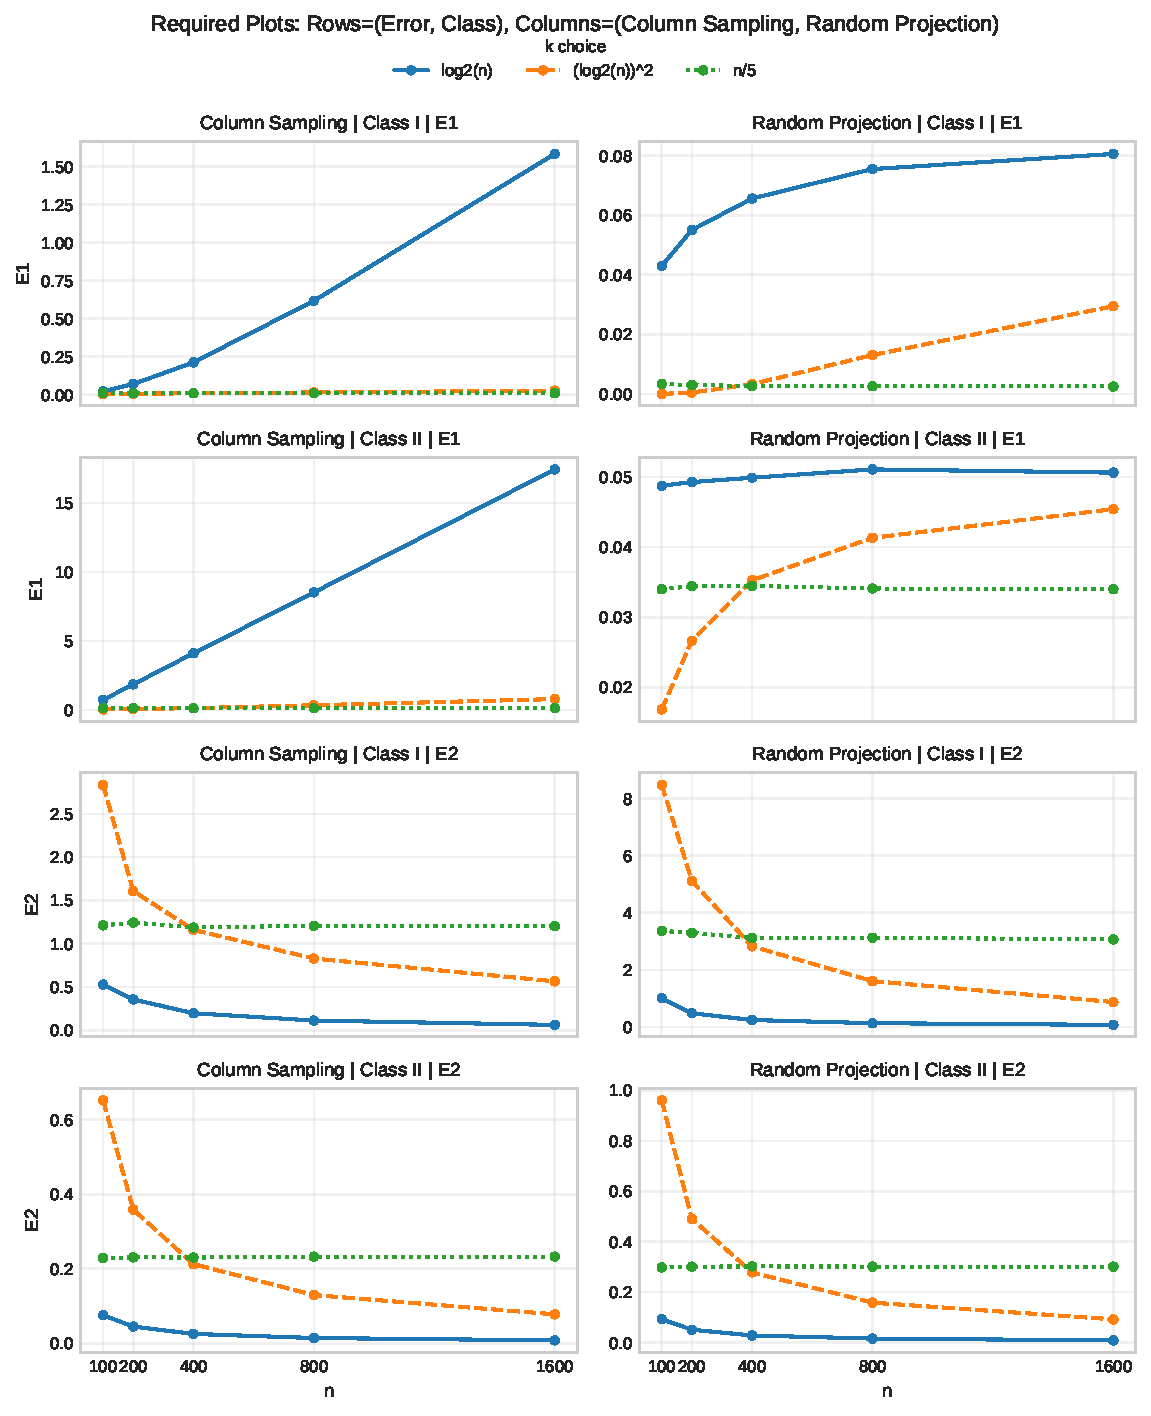
\includegraphics[width=1\textwidth,height=0.78\textheight,keepaspectratio]{required_plots_4x2_a4.pdf}
    \caption{Required plots arranged in a $4\times2$ matrix: each row fixes error-type/class combination, and each column fixes algorithm (left: Column Sampling, right: Random Projection).}
    \label{fig:required_plots_4x2}
\end{figure}

From the next four panels of Figure~\ref{fig:required_plots_4x2} (the two $E_2$ rows), Algorithm 2 generally performs worse (higher $E_2$) than Algorithm 1 for both matrix classes. This behavior is consistent with the implementation choices as described in the problem: Algorithm 1 uses explicit oversampling with $c=2k$, while Algorithm 2 uses a sketch size $\Psi\in\mathbb{R}^{n\times k}$ (i.e., no oversampling beyond $k$). Since $E_2$ depends on subspace reconstruction quality through $\|A-UU^TA\|_F^2$, the extra sampling budget in Algorithm 1 can produce a stronger approximation subspace and hence lower reconstruction error.

Across our experiments, smaller $k$ often gives higher $E_1$ but lower $E_2$.
The reason is that $E_1$ measures accuracy of the estimated top-$k$ singular values directly, and with very small $k$ the estimate is more sensitive to subspace/sampling noise.
In contrast, 
\[
E_2=\frac{\|A-UU^\top A\|_F^2}{\sum_{i=k+1}^n \sigma_i^2}-1
\]
is normalized by the optimal tail energy. For smaller $k$, the denominator $\sum_{i=k+1}^n \sigma_i^2$ is larger, which can make the normalized excess error smaller even when the absolute residual is not smaller.
So this is a normalization-driven trade-off between $E_1$ and $E_2$.

\begin{table}[H]
\centering
\caption{Random Projection wins over Column Sampling by class and $k$-label. } 
\label{tab:rp_vs_cs_wins}
\small
\begin{tabular}{|c|c|c|c|c|c|}
\hline
\textbf{class} & \textbf{$k$\_label} & \textbf{E1\_rp\_wins\_sum} & \textbf{E1\_rp\_win\_\%} & \textbf{E2\_rp\_wins\_sum} & \textbf{E2\_rp\_win\_\%} \\
\hline
I  & $(\log_2(n))^2$ & 4 & 80.0  & 0 & 0.0 \\
I  & $\log_2(n)$     & 4 & 80.0  & 0 & 0.0 \\
I  & $n/5$            & 5 & 100.0 & 0 & 0.0 \\
II & $(\log_2(n))^2$ & 5 & 100.0 & 0 & 0.0 \\
II & $\log_2(n)$     & 5 & 100.0 & 0 & 0.0 \\
II & $n/5$            & 5 & 100.0 & 0 & 0.0 \\
\hline
\end{tabular}
\end{table}

Table~\ref{tab:rp_vs_cs_wins} (where \textbf{E\{1,2\}\_rp\_win\_\%} stands for random projection (Algorithm 2) performing better on E\{1,2\}) confirms the trend from Figure~\ref{fig:required_plots_4x2}: with Algorithm 1 using $c=2k$ and Algorithm 2 using $\Psi\in\mathbb{R}^{n\times k}$, Algorithm 2 is better than Algorithm 1 on $E_1$ in most/all cases, but it gives worse error on $E_2$ in all reported cases.

To make the comparison fairer in sampling budget, we can set $c=k$ for Algorithm 1. In that case, the number of sampled columns in Algorithm 1 is aligned with the sketch width in Algorithm 2 ($\Psi\in\mathbb{R}^{n\times k}$). Under this setting, Algorithm 2 outperforms Algorithm 1 more consistently, including on $E_2$ for most class/$k$-label combinations.

\begin{table}[H]
\centering
\caption{Random Projection wins over Column Sampling when Algorithm 1 uses $c=k$.}
\label{tab:rp_vs_cs_wins_ck}
\small
\begin{tabular}{|c|c|c|c|c|c|}
\hline
\textbf{class} & \textbf{$k$\_label} & \textbf{E1\_rp\_wins\_sum} & \textbf{E1\_rp\_win\_\%} & \textbf{E2\_rp\_wins\_sum} & \textbf{E2\_rp\_win\_\%} \\
\hline
I  & $(\log_2(n))^2$ & 5 & 100.0 & 5 & 100.0 \\
I  & $\log_2(n)$     & 5 & 100.0 & 1 & 20.0  \\
I  & $n/5$            & 5 & 100.0 & 5 & 100.0 \\
II & $(\log_2(n))^2$ & 5 & 100.0 & 5 & 100.0 \\
II & $\log_2(n)$     & 5 & 100.0 & 4 & 80.0  \\
II & $n/5$            & 5 & 100.0 & 5 & 100.0 \\
\hline
\end{tabular}
\end{table}

\subsection{Timing analysis (20-run average)}

To compare computational cost, both algorithms were benchmarked on the same matrix classes and the same $(n,k)$ grid, and each case was averaged over 20 runs.
Figure~\ref{fig:timing_20runs} shows the mean runtime trend versus $n$ (for k = $(\log_2 n)^{2}$) for Class I and Class II.

From this timing benchmark, Algorithm 2 (Random Projection) takes more time on average than Algorithm 1 (Column Sampling).
Hence, in this implementation, Algorithm 1 is the faster method while Algorithm 2 is computationally heavier.

\begin{figure}[H]
    \centering
    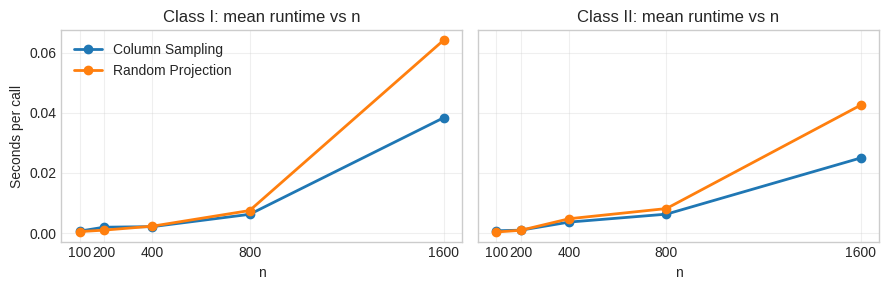
\includegraphics[width=0.95\textwidth]{times.png}
    \caption{Mean runtime vs. $n$ for both matrix classes, using 20-run averages.}
    \label{fig:timing_20runs}
\end{figure}

\begin{figure}[H]
    \centering
    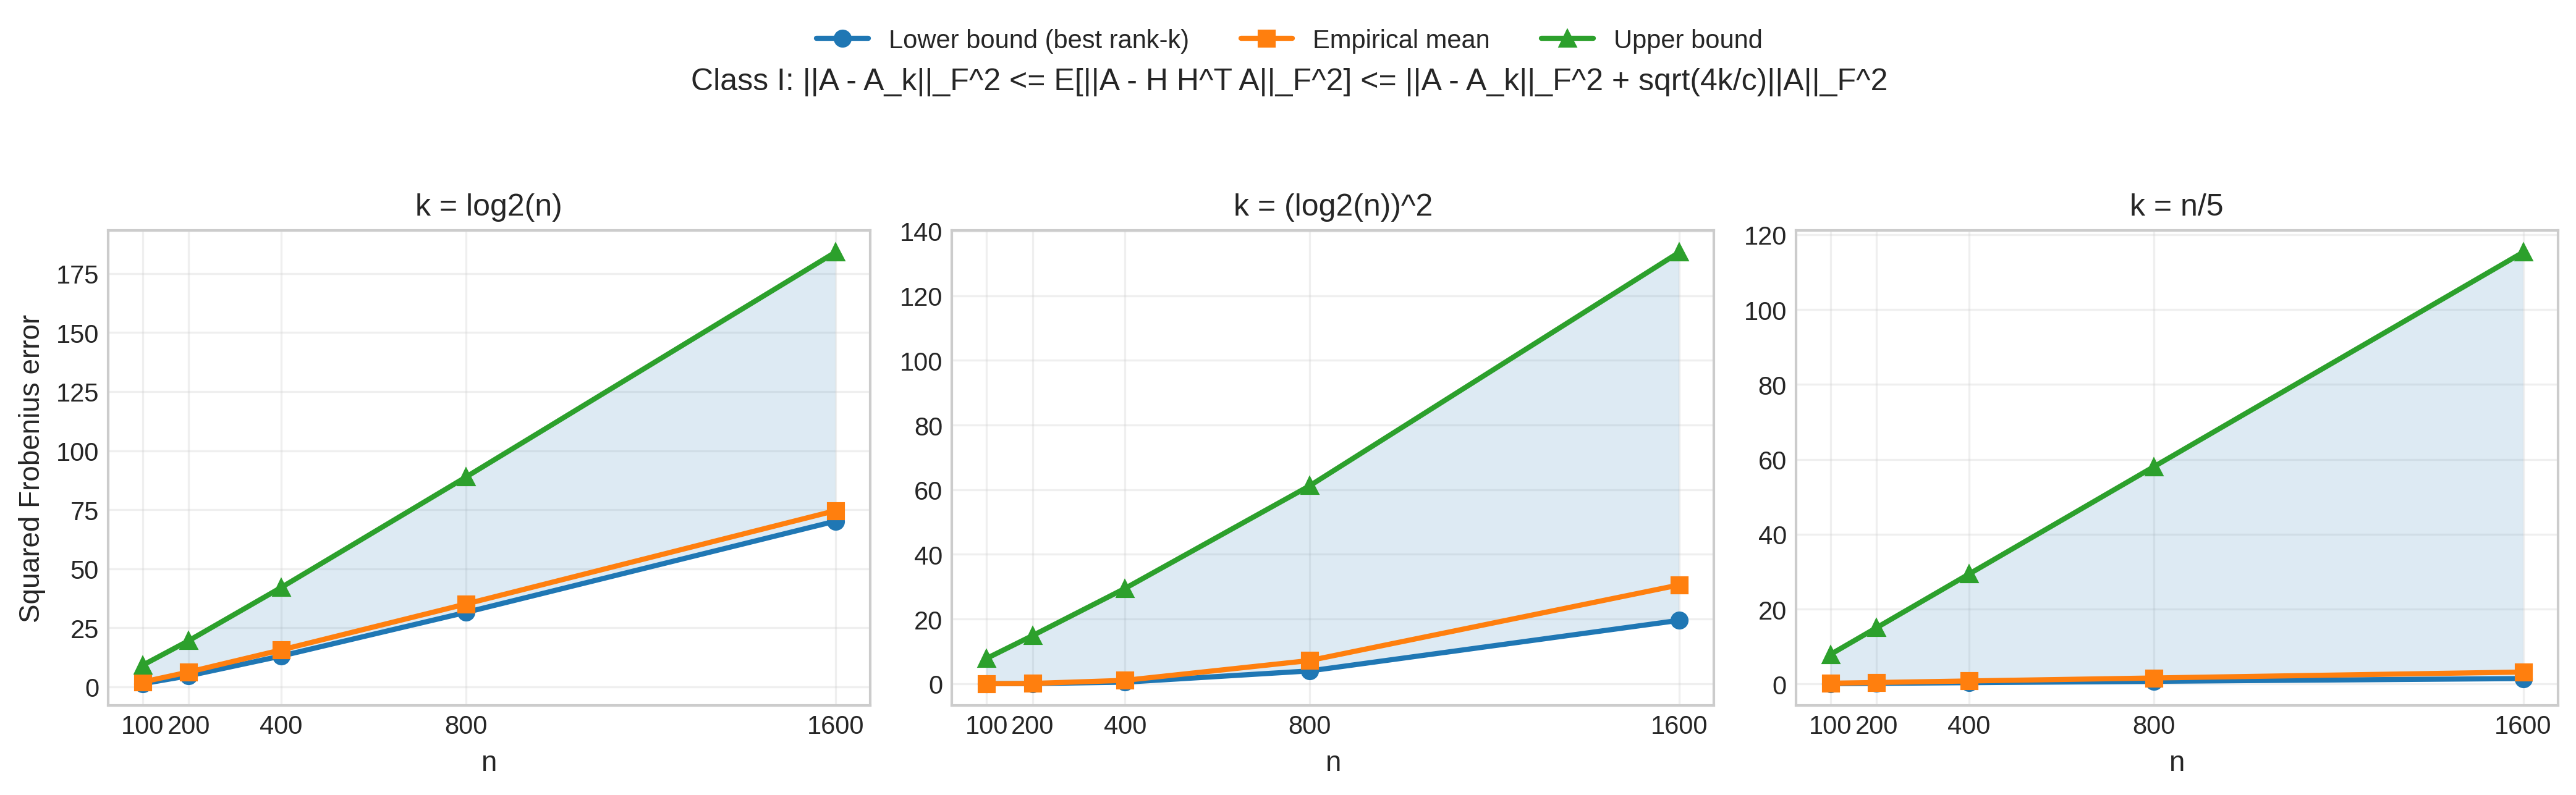
\includegraphics[width=1\textwidth]{bounds_class_I_fro.png}

    \vspace{0.6em}
    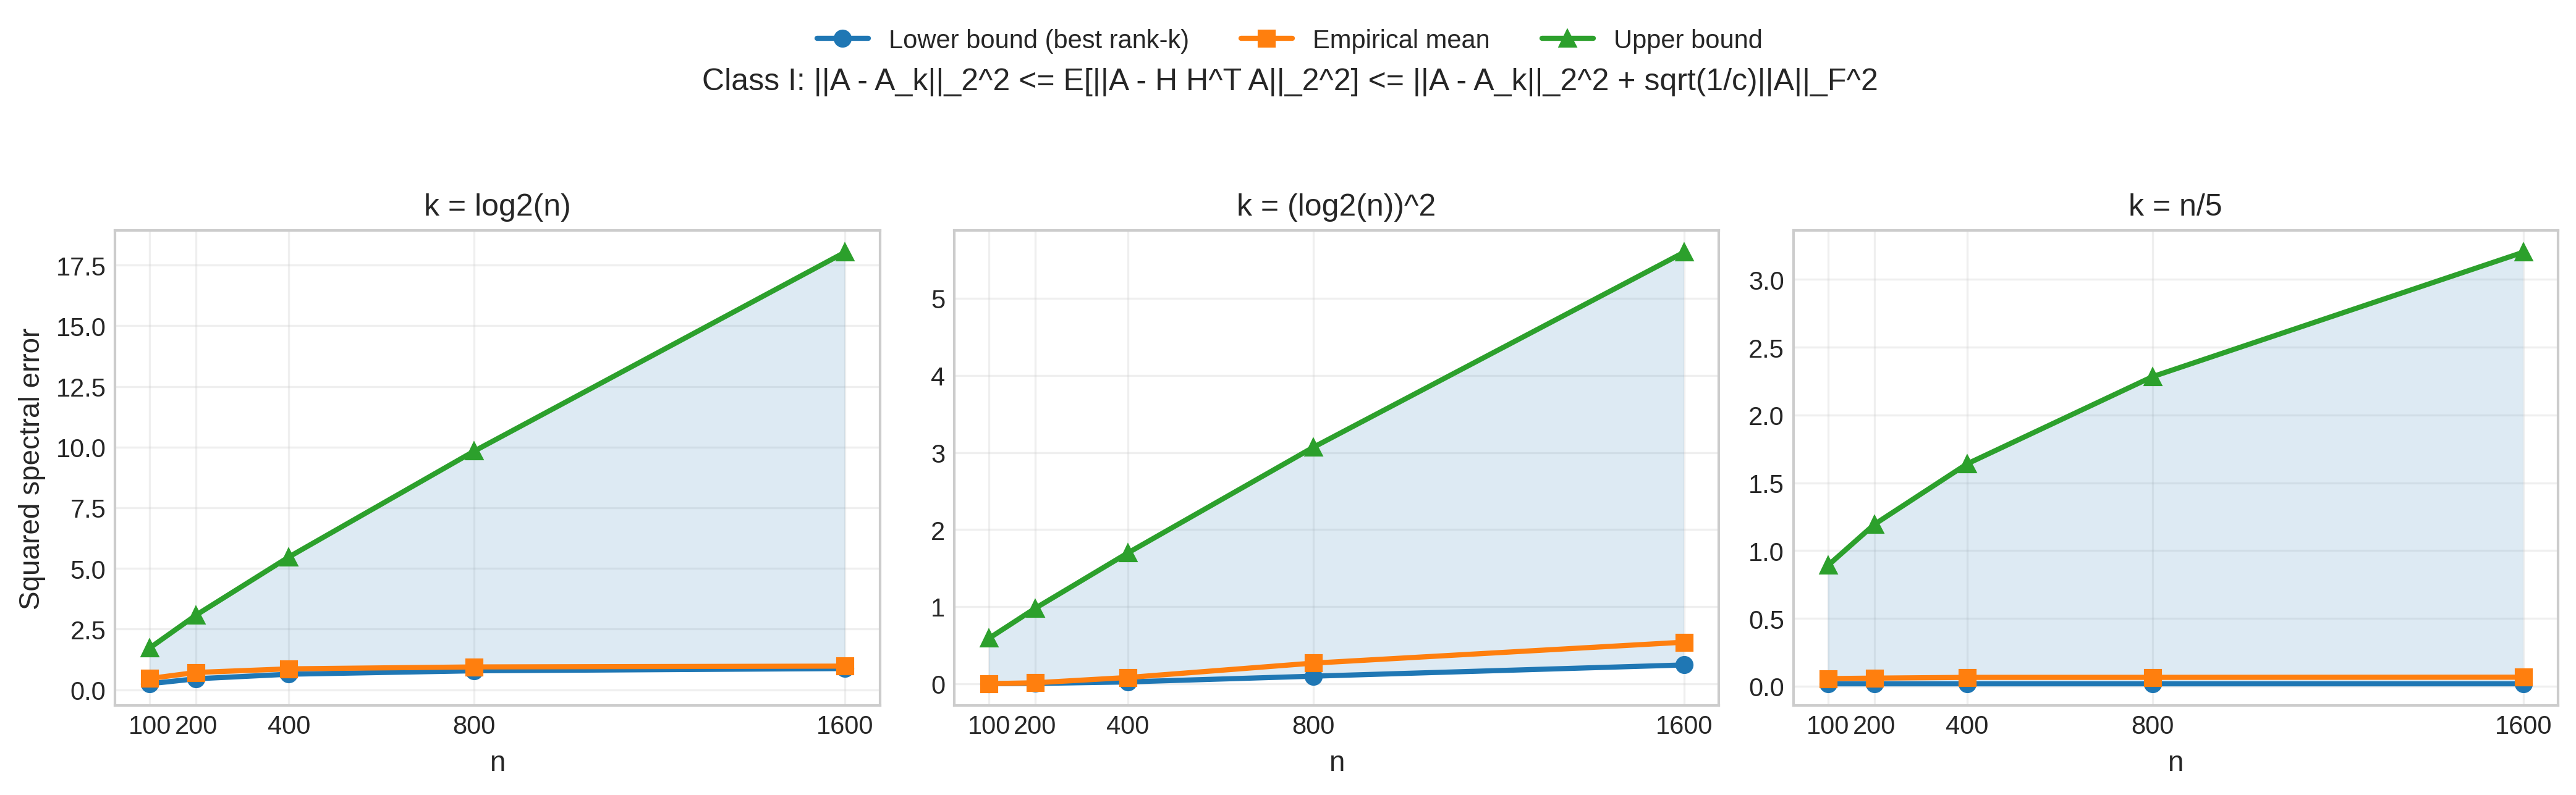
\includegraphics[width=1\textwidth]{bounds_class_I_op.png}

    \vspace{0.6em}
    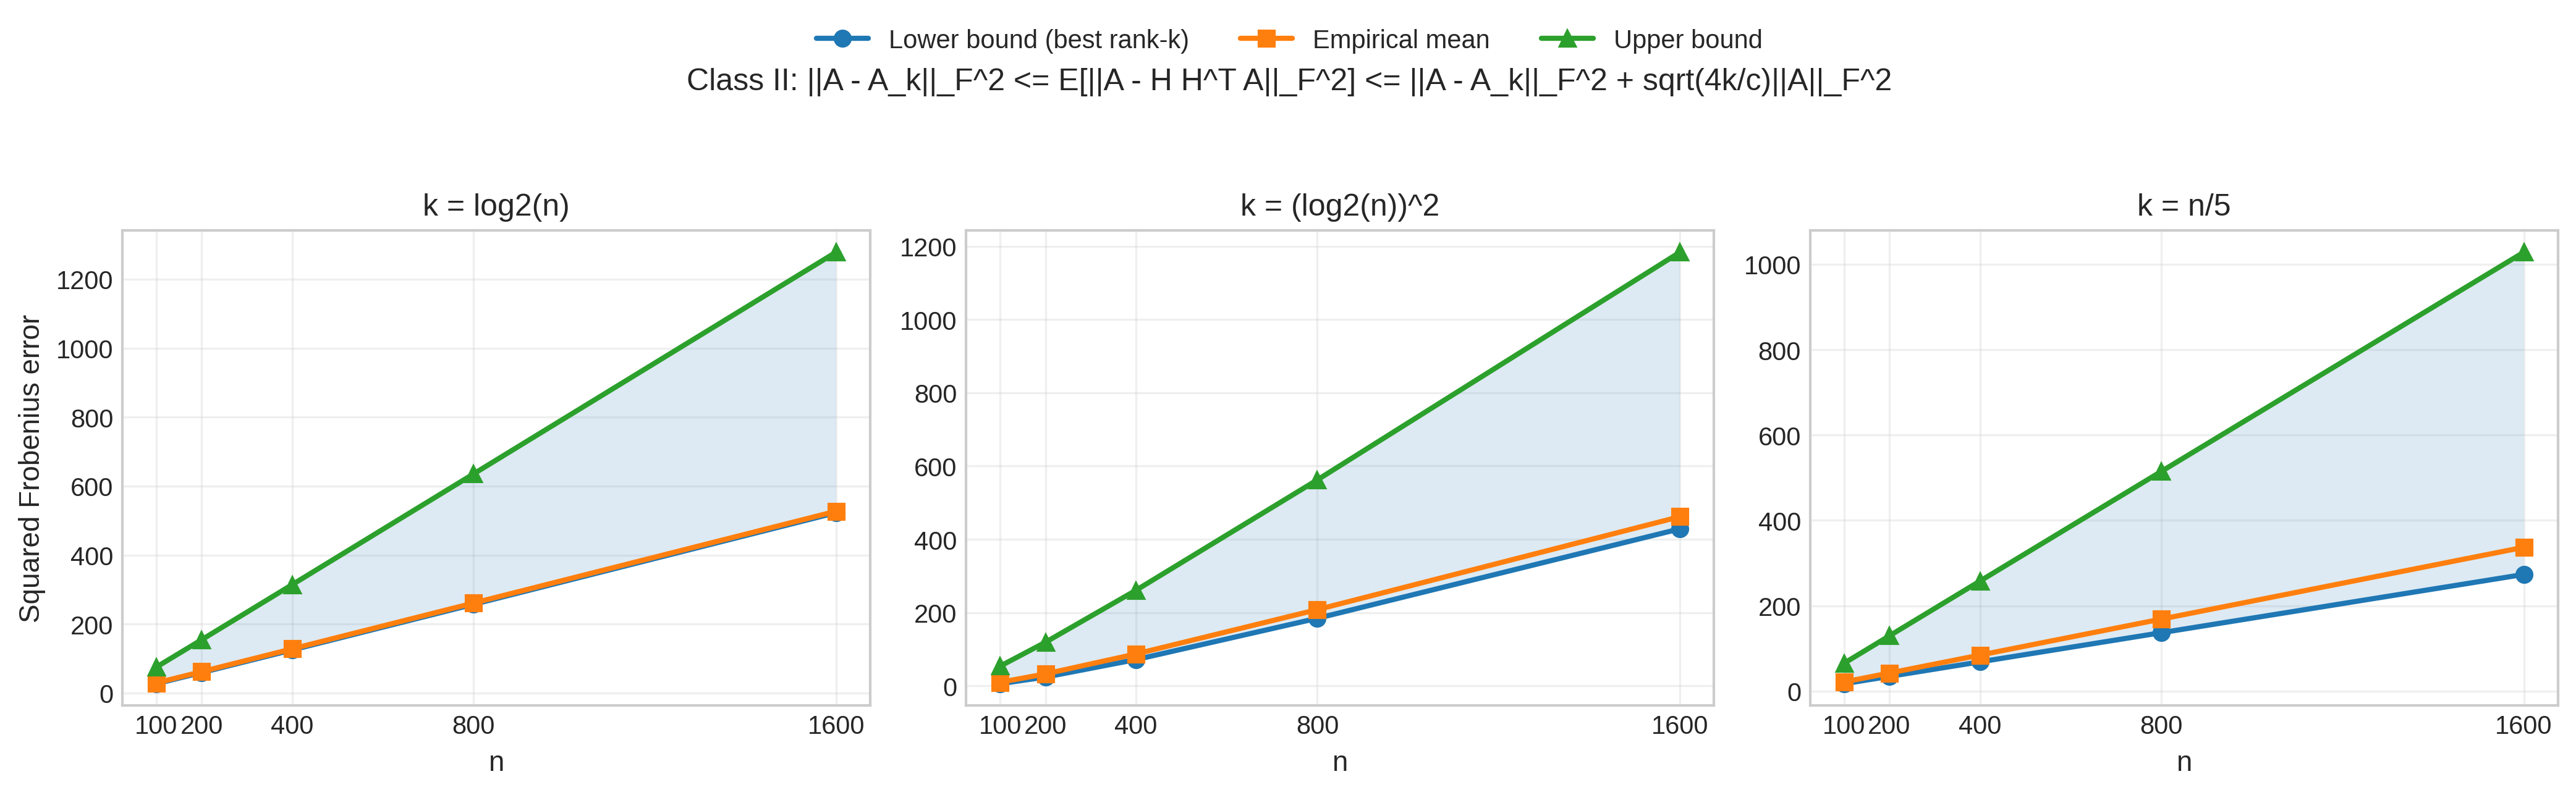
\includegraphics[width=1\textwidth]{bounds_class_II_fro.png}

    \vspace{0.6em}
    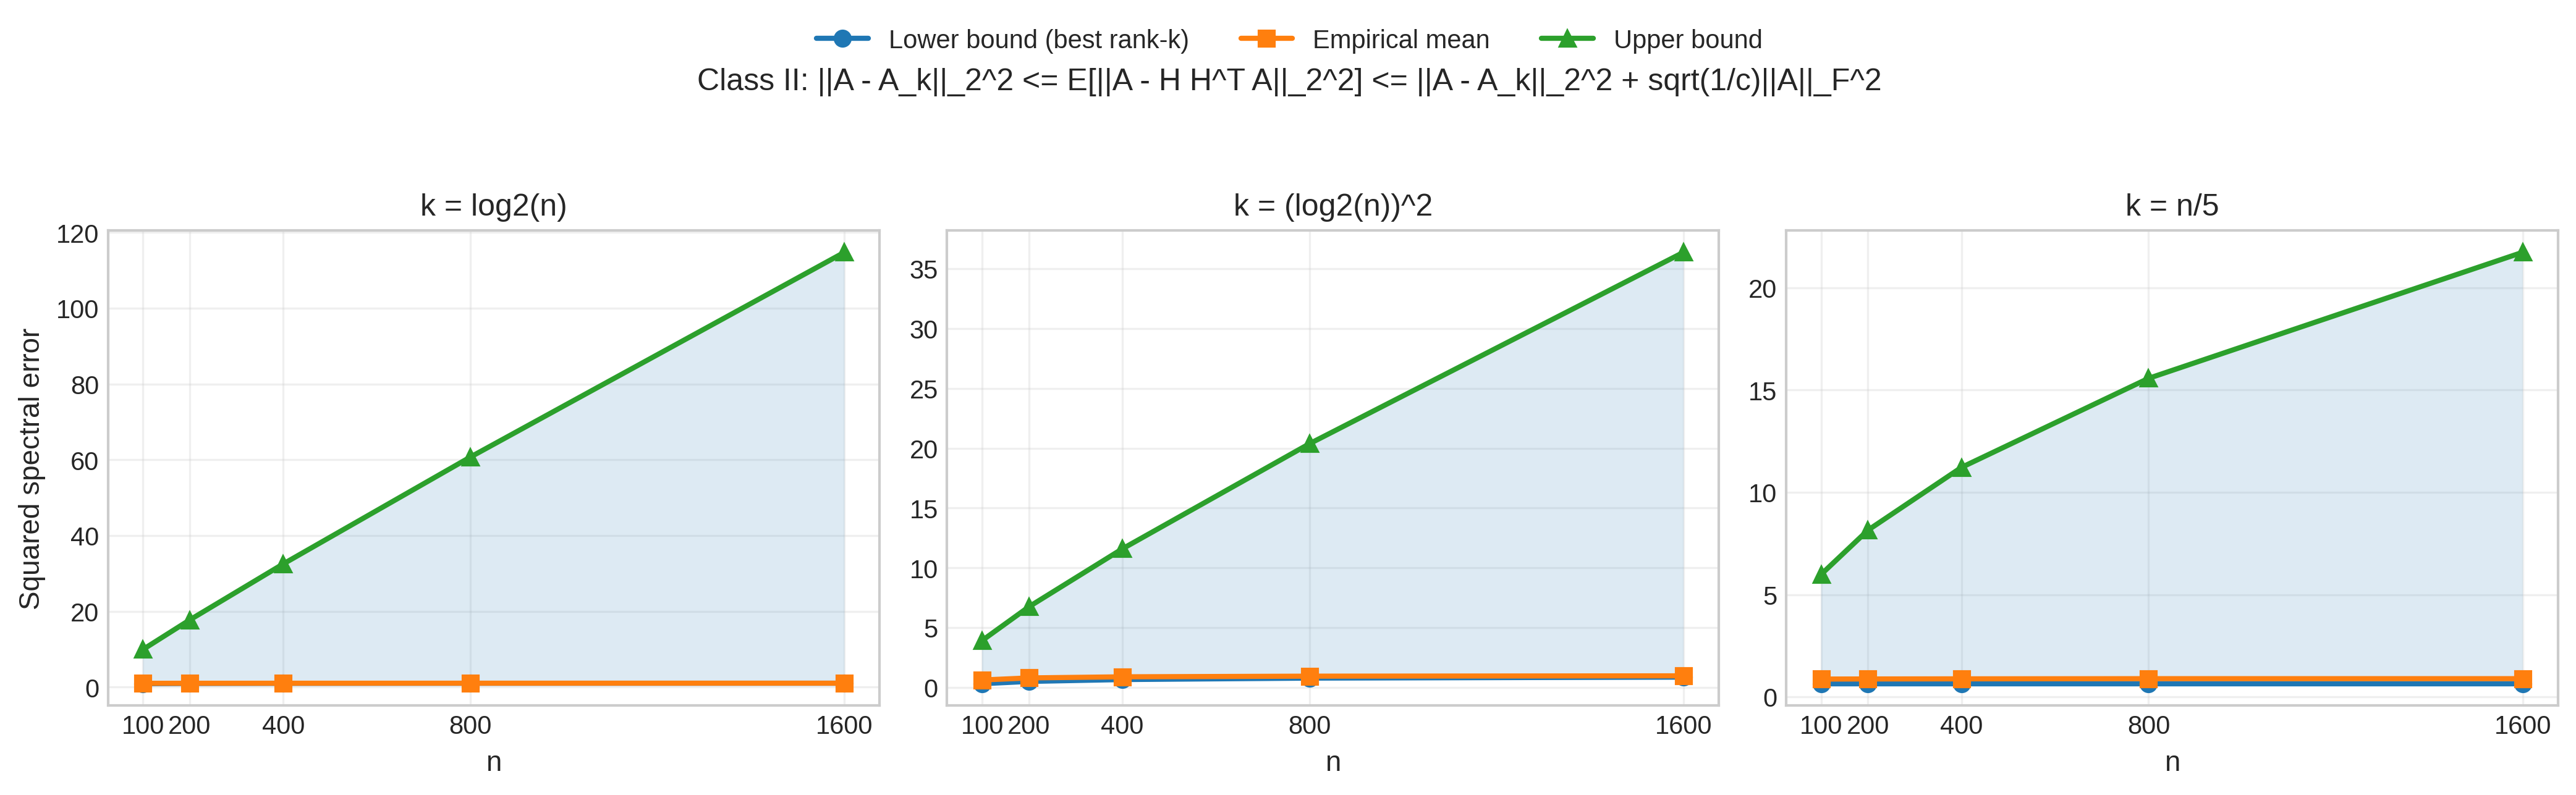
\includegraphics[width=1\textwidth]{bounds_class_II_op.png}
    \caption{Bound-verification plots shown vertically (top to bottom): Class-I/Frobenius, Class-I/Spectral, Class-II/Frobenius, and Class-II/Spectral.}
    \label{fig:bounds_class_stack}
\end{figure}

\subsection{Stability verification using coefficient of variation}

As discussed in class, Algorithm 2 is expected to be more stable than Algorithm 1. We verify this by comparing the coefficient of variation values computed from repeated runs.

\begin{figure}[H]
\centering
\begin{minipage}[t]{0.58\textwidth}
\vspace{0pt}
For both matrix classes and for both error metrics, Random Projection (Algorithm 2) has smaller CV than Column Sampling (Algorithm 1). This means Algorithm 2 has lower relative dispersion across runs and is empirically more stable.

In Class I, CV ranges from $(0.2208, 0.0960)$ to $(0.1006, 0.0602)$ for $(E_1, E_2)$. In Class II, CV ranges from $(0.1013, 0.0324)$ to $(0.0338, 0.0157)$. These results are consistent with the classroom claim that Algorithm 2 is more stable.
\end{minipage}\hfill
\begin{minipage}[t]{0.40\textwidth}
\vspace{0pt}
\centering
\small
\begin{tabular}{|c|c|c|}
\hline
\textbf{Class} & \textbf{Algorithm} & \textbf{E1\_cv / E2\_cv} \\
\hline
I  & Column Sampling   & 0.2208 / \textbf{0.0960} \\
I  & Random Projection & 0.1006 / \textbf{0.0602} \\
II & Column Sampling   & 0.1013 / \textbf{0.0324} \\
II & Random Projection & 0.0338 / \textbf{0.0157} \\
\hline
\end{tabular}
\captionof{table}{Average coefficient of variation by class and algorithm. Lower is more stable.}
\label{tab:cv_stability_summary}
\end{minipage}
\end{figure}

\subsection{Experimental verification of convergence bounds}


In class, the convergence bounds for Algorithm 1 were discussed in both Frobenius and spectral norms. We verify these bounds experimentally by averaging over randomized column-sampling runs and comparing three quantities for each setting: (i) the lower bound (best rank-$k$ error), (ii) the empirical mean error, and (iii) the theorem upper bound.

The two bounds verified are:
\[
\|A-A_k\|_F^2 \le \mathbb{E}\|A-HH^TA\|_F^2 \le \|A-A_k\|_F^2 + \sqrt{\frac{4k}{c}}\,\|A\|_F^2,
\]
\[
\|A-A_k\|_2^2 \le \mathbb{E}\|A-HH^TA\|_2^2 \le \|A-A_k\|_2^2 + \sqrt{\frac{1}{c}}\,\|A\|_F^2.
\]

Figure~\ref{fig:bounds_class_stack} shows the updated bound-verification plots using all notebook $n$ values:
\[
n\in\{100,200,400,800,1600\}.
\]
Across all panels, the empirical mean remains within the theoretical interval, validating the bounds in practice for the full tested grid.

From the code provided in notebook attached, all bound-check flags evaluate to true for the tested cases:
\[
\texttt{all\_bounds\_ok=True for }30/30\text{ cases}.
\]
Hence, the lower and upper inequalities hold in both Frobenius and spectral forms for every tested $(\text{class},n,k)$ setting.

An important qualitative observation is that the empirical mean curve is typically much closer to the lower bound than to the upper bound. This indicates that, while the upper bound is valid, it is conservative; practical performance is significantly better than the worst-case guarantee.

\section{Conclusion}

This work compared column sampling (Algorithm 1) and random projection (Algorithm 2) for top-$k$ singular-component estimation across matrix classes I and II and multiple $n,k$ settings. The experiments show that Algorithm 2 is generally more accurate for singular-value estimation ($E_1$), while reconstruction behavior ($E_2$) depends on sampling-budget fairness: with $c=2k$ for Algorithm 1, Algorithm 1 can be more favorable on $E_2$, whereas under the fairer setting $c=k$, Algorithm 2 improves consistently and wins in most cases.

Runtime benchmarking shows that Algorithm 2 is computationally heavier on average than Algorithm 1 in this implementation. Stability analysis using the coefficient of variation confirms the class discussion: Algorithm 2 has lower run-to-run variability than Algorithm 1 for both matrix classes and both error metrics. Finally, empirical verification of the Frobenius and spectral convergence bounds confirms that all tested cases satisfy the theoretical inequalities, with empirical means typically much closer to the lower bound than the upper bound, indicating conservative but valid upper guarantees.



\end{question}

\end{document}